% ============================================================
\subsection{mLogistics / LoApp}
% ============================================================
Die Hauptapplikation, mLogistics oder auch LoApp genannt, setzt, wie alle Serverseitigen Applikationen von LogObject auf die Libary log4J. mLogistics enthält die Businesslogik und generiert Logs die zur Fehlerlösung und Überwachung ebenjener genutzt werden können.

\subsubsection{Konfiguration}
Das Logging in der Hauptapplikation ist zentralisiert, das heißt das alle Nodes des Clusters die Logs an eine Node senden welche die Logs schreibt. Es ist möglich zusätzlich eine Node als sekundäre Node zu definieren, welche im Fall eines Ausfalls der primären Node, das Loggen übernimmt. (Referenz zu Abschnitt einfügen)
Die Logdateien werden in einem lokalem Speicher abgespeichert. \\

Für die Konfiguration des Loggings gibt es Konfigurationsdateien: \textit{log4j2.xml} und \textit{logserver2.xml}.
Für die Konfiguration des mLogistics-Loggings gibt es zwei Konfigurationsdateien: \textit{log4j2.xml} und \textit{logserver2.xml}. Für die Hauptapplikation werden zwei getrennte genutzt um die Appenders von den Loggern zu trennen. So ist die Konfiguration übersichtlicher.

\paragraph{Konfigruationsdatei}
\vspace{0.5em}
\begin{quote}
	Konfiguration Appenders: \textit{~/cfg/log4j2.xml} \\
	Konfiguration Pfade und Logs: \textit{~/cfg/logserver2.xml}
\end{quote}

\textbf{log4j2.xml} \\
Der Inhalt der \textbf{log4j2.xml} Datei kann in dem Kapitel \textit{\nameref{subsec:mlogistics_log4j2_config}} eingesehen werden.

\textbf{logserver2.xml} \\
Der Inhalt der \textbf{logserver2.xml} Datei kann in dem Kapitel \textit{\nameref{subsec:mlogistics_logserver2_config}} einesehen werden.

\paragraph{Start/Stop des Logging}
Der Loggingservice kann mit Befehlel getartet und gestoppt werden.
\begin{quote}
	Start des Logginservices: \textit{~/server/bin/mlogistics startlog}\\
	Beenden des Logginservices: \textit{~/server/bin/mlogistics stoplog}
\end{quote}



\subsubsection{Serverlogs}

%------------------------------------------------
%	Logconfiguration
%------------------------------------------------

%------------------------------------------------
%	Access Log
%------------------------------------------------
\paragraph{\mlogisticsAccessLog}
Das \texttt{\mlogisticsAccessLog} enthält Informationen über Zugriffe von Usern auf die Clients, also mRic und MOT.

%------------------------------------------------
%	Alivelog
%------------------------------------------------
\paragraph{\mlogisticsAliveLog}
Das \texttt{\mlogisticsAliveLog} enthält Daten zum Workplacemanagement.

%------------------------------------------------
%	Auditlog
%------------------------------------------------
\paragraph{\mlogisticsAuditLog}
Das \texttt{\mlogisticsAuditLog} enthält drei Ebenen von Logs für sicherheitsrelevante und betrieblich signifikante Ereignisse im System.
\begin{itemize}
	\item \textbf{AUTH} (Info-Level): Protokolliert Login-Versuche und erfolgreiche Anmeldungen.
	\item \textbf{SEC} (Warn-Level): Protokolliert potenzielle Sicherheitsvorfälle, wie unautorisierte Zugriffsversuche auf Daten oder fehlgeschlagene Logins.
	\item \textbf{OPS} (Debug- und Info-Level): Protokolliert die vom Benutzer ausgeführten Transaktionen und Operationen.
\end{itemize}

%------------------------------------------------
%	Commandinglog
%------------------------------------------------
\paragraph{\mlogisticsCommandingLog}
Das \texttt{\mlogisticsCommandingLog} was introduced for this ticket https://redmine.logobject.ch/issues/60450, but it is implemented only on TCS level.

%------------------------------------------------
%	Commanding Cache Log
%------------------------------------------------
\paragraph{\mlogisticsCommandingCacheLog}
Das \texttt{\mlogisticsCommandingCacheLog} ist das Commanding Resource.

%------------------------------------------------
%	Commanding Debug Log
%------------------------------------------------
\paragraph{\mlogisticsCommandingDebugLog}
Das \texttt{\mlogisticsCommandingDebugLog} ist für TCS implementiert worden.

%------------------------------------------------
%	CXF log
%------------------------------------------------
\paragraph{\mlogisticsCxfLog}
Das \texttt{\mlogisticsCxfLog}  Protokolliert alle Webdienste, die die Apache CXF-Bibliothek verwenden, von denen es auf allen Ebenen viele gibt, beispielsweise MFJ (interner Dienst), aber auch GDI (externe und SNDE-Ebene).

%------------------------------------------------
%	Errorlog
%------------------------------------------------
\paragraph{\mlogisticsErrorLog}
Das \texttt{\mlogisticsErrorLog} sammelt alle Logs mit dem Level \texttt{ERROR} oder höher. Sie dient dazu, kritische Fehlerzustände des Systems gezielt nachzuverfolgen.

%------------------------------------------------
%	GDI-Importlog
%------------------------------------------------
\paragraph{\mlogisticsGdiImportLog}
Das \texttt{\mlogisticsGdiImportLog} Protokolliert nur Vorgänge, die mit GDI (SNDE-Level-Schnittstelle) stattfinden, insbesondere importAlarmObjects, importLayers, importDivisions.

%------------------------------------------------
%	Lockinglog
%------------------------------------------------
\paragraph{\mlogisticsLockingLog}
Das \texttt{\mlogisticsLockingLog} enthält Informationen über den Lockingmechanismus.

%------------------------------------------------
%	MOTlog
%------------------------------------------------
\paragraph{\mlogisticsMotLog}
Das \texttt{\mlogisticsMotLog} enthält Informationen über die interaktionen des Server mit der MOT.

%------------------------------------------------
%	MOT Formslog
%------------------------------------------------
\paragraph{\mlogisticsMotFormsLog}
Das \texttt{\mlogisticsMotFormsLog} enthält Informationen über die Synchronisation der MOT Forms.

%------------------------------------------------
%	Multiqueryservletlog
%------------------------------------------------
\paragraph{\mlogisticsMultiQueryServletLog}
Das \texttt{\mlogisticsMultiQueryServletLog} enthält wie auch das \mlogisticsQueryServletLog und das \mlogisticsQueryStreamLog informationen über Queries die durch mRic ausgehen.

%------------------------------------------------
%	PushD
%------------------------------------------------
\paragraph{\mlogisticsPushDLog}
Das \texttt{\mlogisticsPushDLog} protokolliert die Operationen, die über die PushD-Funktionalität ausgeführt werden.

%------------------------------------------------
%	Queryservletlog
%------------------------------------------------
\paragraph{\mlogisticsQueryServletLog}
Das \texttt{\mlogisticsQueryServletLog} enthält wie auch das \mlogisticsMultiQueryServletLog und das \mlogisticsMultiQueryServletLog informationen über Queries die durch mRic ausgehen.

%------------------------------------------------
%	Querystreamlog
%------------------------------------------------
\paragraph{\mlogisticsQueryStreamLog}
Das \texttt{\mlogisticsQueryStreamLog} enthält wie auch das \mlogisticsQueryServletLog{} und das \mlogisticsQueryStreamLog{} Informationen über Queries die durch mRic ausgehen.

%------------------------------------------------
%	Schedulerlog
%------------------------------------------------
\paragraph{\mlogisticsSchedulerLog}
Das \texttt{\mlogisticsSchedulerLog} enthält die Logs des Schedulers

%------------------------------------------------
%	Serverlog
%------------------------------------------------
\paragraph{\mlogisticsServerLog}
Das \texttt{\mlogisticsServerLog} enthält alle Logs, die in den anderen Logdateien nicht erfasst werden. Sie bezieht sich hauptsächlich auf serverbezogene Ereignisse.

%------------------------------------------------
%	Warnlog
%------------------------------------------------
\paragraph{\mlogisticsWarnLog}
Das \texttt{\mlogisticsWarnLog} enthält alle Logs auf Warn-Level. Es erfolgt keine inhaltliche Filterung, sondern lediglich eine Selektion nach Log-Level.




\paragraph{\mlogisticsLogserverLog}
Das \texttt{\mlogisticsLogserverLog} ist das Log des Logservers selbst. In einer Cluster-Umgebung gibt es einen zentralen Server, der alle Events der Umgebung sammelt. Dieses Log dokumentiert speziell die Aktivitäten des Logservers.

\subsubsection{mRic/Web Logs}
Die Logs die der Web-Client in der Runtime generiert wird nur bei Bedarf an den Server gesendet und gespeichert. Zum Senden der Log wird die \textit{Send Log} Funktion in dem Webclient ausgeführt. (Welches Grant?) (Wo kann man die Einsehen?)

\begin{figure}[h]
	\centering
	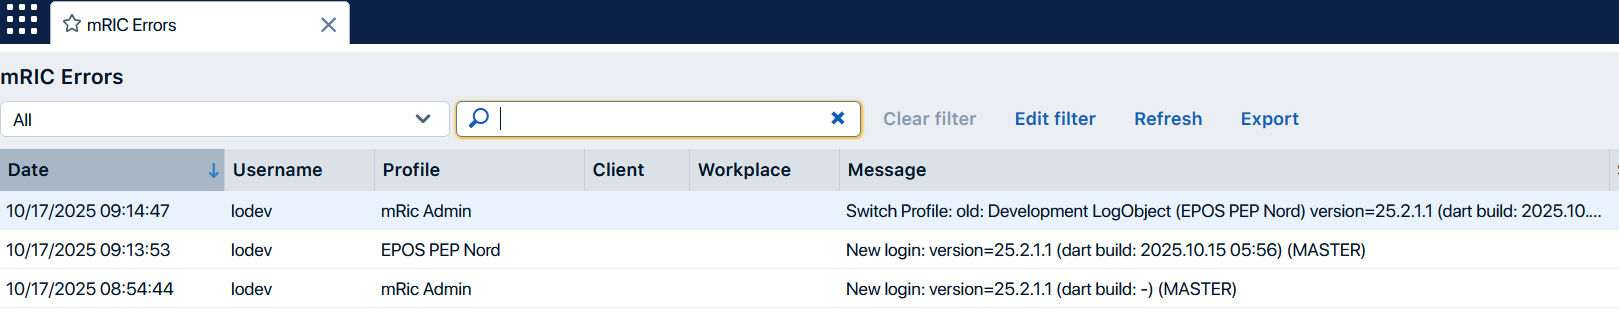
\includegraphics[width=1\linewidth]{./attachements/mricerrorlog.png}
	\caption{mRic Errors}
\end{figure}
